\chapter{Methodology}
\label{sec:methodology}

%%%%%%%%%%%%%%%%%%%%% Kurze Einführung %%%%%%%%%%%%%%%%%%%%%

In this section, the methodology of this work is described.
In <section> used and implemented models are explained.
<section> describes datasets, which are used to train and evaluate models and other algorithms.
The data augmentation of these datasets is depicted in <section>.
<section> deals with loss functions. After that, setups for training and inference measurements are described in <section> and <section>.
Keep in mind that the main contributions of this work include three parts:
%1. an initial approach to combine object detection with semantic segmentation;
%2. TEP-Net \cite{tepNet2024} is the new baseline for further experiments to improve this model's accuracy and robustness;
%3. An RNN is integrated into the model to increase robustness further;

\begin{enumerate}
    \item An initial approach to combine object detection with semantic segmentation.
    \item TEP-Net \cite{tepNet2024} is the new baseline for further improvements in accuracy and robustness.
    \item An RNN is integrated aiming to eliminate the limitation of single-frame-based approaches.
\end{enumerate}

%%%%%%%%%%%%%%%%%%%%%%%%%% Models %%%%%%%%%%%%%%%%%%%%%%%%%%

%\input{methodology/yolo_models.tex}
\section{Models}

In this section all models are discussed which are used or created in this work.
This section is divided into three subsections.
Each of them corresponds to one of the main contributions of this work.
Therefore the first section gives a brief overview of used object detection models, the second one with the \ac{TEP}-Net \cite{tepNet2024} because it is used as a baseline.
Additionally, further improvements of this model are described in this section.
The last section describes all temporal models.

\subsection{Object Detection Models}

The state of the art in \autoref{sec:ObjectDetection} shows that one-stage detectors have the most promising characteristics to be successfully utilized in this work.
The most interesting ones are the models from the \ac{YOLO} series, especially the most recent ones because they focus on improved parameter usage.
This makes the models light weight and presents an advantage for this work, because operation on limited hardware is aimed for.
At the start of this work the most recent model from the \ac{YOLO} series is the \ac{YOLO}v9 \cite{YOLOv9}.
For object detection different models of the \ac{YOLO}v9 and the \ac{GELAN} series are available.
However, the \ac{YOLO}v9 models were not fully supported at that time.
Therefore the models used for experiments include the \ac{GELAN}-c and \ac{GELAN}-e.
These are obtained trough the GitHub repository \cite{YOLOv9GitHub} and used unchanged.
An additional model which is used for experiments is the \ac{YOLO}v7 \cite{yolov7} model, which is also utilized unchanged from the GitHub repository \cite{YOLOv7GitHub}.

\subsection{TEP-Net Model}
\label{subsec:baselineModel}

In the literature rails are often detected without distinction between all rails visible in an image and the rail the train continues.
\cite{tepNet2024} therefore proposes a regression-based approach, which restricts the model to predict a single track.
The idea comes from various lane detection methods in autonomous driving applications for road cars and is fitted the rail domain.

Although rails can be represented by second or third-degree polynomials in curves \cite{PolyLaneNetRoad2021}, they may also take more complex geometric shapes.
Hence, limiting the output to presumed forms is discouraged.
Therefore, the method used in \cite{tepNet2024} employs spline interpolation to describe such complex structures.

\begin{figure}[H]
    \centering
    \includegraphics[width=\linewidth]{PICs/Baselinepaper/TEP-Net_model.jpg}
    \caption{\ac{TEP}-Net model architecture\cite{tepNet2024}. The input of the model is a cropped and resized image and the output of the model are the $x$-values for the left and right rail on each anchor line plus an additional value for the $y$-limit.}
    \label{fig:TEP-Net_model}
\end{figure}

As shown in the prediction of \autoref{fig:TEP-Net_model}, a set of horizontal lines are overlayed in the cropped image.
The number of $y$-lines or "anchors" is determined by a hyperparameter.
They are uniformly distributed along the $y$-axis. For each line, two $x$-values are predicted.
One for the left rail and one for the right rail.
The second and fourth images in the bottom row of \autoref{fig:tepNet_dataaugmentation} and the prediction image of \autoref{fig:TEP-Net_model} show that rails do not necessarily cross with anchor lines at the top of image crops.
Therefore, an additional $y$-limit is predicted, which gives information up to which anchor the rail should be detected.
Anchors and their $x$-values above this horizon line do not hold valuable information and are ignored.

For this novel regression task, a new model architecture is created.
For this model widely used backbone architectures like ResNet and EfficientNet are chosen.
These backbones extract relevant features from the cropped images reducing the spatial dimensions and increasing channel size to a high number.
After that, the feature map's number of channels is reduced to a predefined size with a 1x1 Conv2d layer \cite{pytorch_conv2d_docu} and flattened to a vector.
This feature vector serves as the input for the prediction head, which consists of two fully connected layers \cite{pytorch_linearLayer_docu} in series.
The size of the linear layers is set with a hyperparameter.
In the last layer, a reduction leads to the resulting prediction vector with the dimension $2 \times H + 1$.
$H$ is the number of anchors.
This vector includes the entire information of one prediction.
The first set of values with size $H$ is for the left rail, another $H$ set for the right rail and the $+ 1$ is for the last values being the horizon line.

This architecture's policy for value ranges does not restrict the $x$-values in any way.
This way predictions can be outside of a crop and the model can learn that sometimes the rails extend out of the viewed field.
The $y$-limit on the other hand is constrained to a range between 0 and 1 with a Sigmoid function.

The introduced model architecture can be classified as an end-to-end framework.
This means the model can be trained and used for inference without any steps in between.
It takes in raw data and results in a complete prediction.

% Improvements to baseline model
%\input{methodology/temporal models.tex} + dataloading

%%%%%%%%%%%%%%%%%%%%%%%%% Datasets %%%%%%%%%%%%%%%%%%%%%%%%%

% RailSem19 for Yolos + used subsets [1/2 bis 1 Seite]
% TEP-annotations [1/2 Seite bzw. ein kurzer Absatz]
% Switch evaluation dataset (all images with switches from val and test dataset) [1/2 Seite bzw. ein kurzer Absatz]
% auto labler + temporal dataset + dass ich CVAT versendet habe[1 bis 2 Seiten]

\section{Datasets}
\label{sec:usedDatasets}

In this section all datasets are described that are used in this work.
The first subsection describes which subsets of RailSem19 are used for the first attempt for the training of object detection models.
Then the annotations of \cite{tepNet2024} are briefly discussed, which are used to train all single-frame-based models.
After that a switch evaluation dataset is described that is used to evaluate singe-frame models on switch scenarios.
The last subsection deals with the temporal dataset and its creation.


\subsection{RailSem19 and subsets for training object detection models}

The first approach to creating a Rail Track Prediction system includes combining an object detection model with a semantic segmentation model.
Since RailSem19 supports both of these methods this dataset is chosen for training.
Furthermore, state-of-the-art research in \autoref{sec:datasets} shows that this dataset is the only one that not only includes switch annotations but also labels for switch states: $switch\_left$, $switch\_right$.
Since not all states are identifiable even though a switch is visible there also is the $switch\_unknwon$ label.

In this work, the bounding boxes are utilized to train the \ac{YOLO} object detection models.
Experiments have been conducted with three versions of this dataset.
An overview of these subsets is shown in \autoref{tab:usedSubsetsforYOLOs}.
The first set is the whole dataset, which includes 8500 images with all different bounding box labels.
The second subset only considers images with switch labels including the $switch\_unknown$ label.
For this subset, 2764 images remain. The third subset only considers the switch labels in which the state is identifiable.
This is because when focusing on the train's direction, the $switch\_unknown$ label does not hold any valuable information.
To prevent confusion, all images containing $switch\_unknown$ annotations are intentionally excluded, resulting in a final set of 1,240 images.

\begin{table}[H]
    \centering
    \begin{tabular}{|l|l|l|}
    %\begin{tabular}{| p{0.3\linewidth} | p{0.6\linewidth} |}
        \hline
        \textbf{RailSem19} & \textbf{RailSem19\_onlySwitches} & \textbf{RailSem19\_onlySwitchesLeftRight}\\
        \hline
        8500 images & 2764 images & 1240 images\\
        \hline
        all bounding box labels & $switch\_left$ & $switch\_left$\\
        \hline
        & $switch\_right$ & $switch\_right$\\
        \hline
        & $switch\_unknown$ & images with $switch\_unknown$ excluded\\
        \hline
    \end{tabular}
    \caption{Used dataset subsets of RailSem19 for training \ac{YOLO} object detection models}
    \label{tab:usedSubsetsforYOLOs}
\end{table}

Since the experiments of training object detection models showed unsatisfactory results also described in <section>, this methodology was deemed ineffective.
This leads to the pursuit of a different solution and experiments with semantic segmentation models are therefore not accomplished.
Consequently the corresponding dense labels of the RailSem19 dataset are not utilized.

\subsection{TEP annotations}

For training single-frame-based models \cite{tepNet2024} published its annotations for the images of RailSem19.
These annotations consist of polylines for the left and the right rail of the train.
Only the two rails are included in the labels which the train drives on.
This is also the case when switches are present.
Additionally, some images are excluded from this dataset when the train's track is not identifiable.
For labeling this dataset the online tool CVAT \cite{cvat} is used.
These annotations can then be transformed with pre processing step to support other models like semantic segmentation. 
This dataset is described in more detail in \autoref{subsubsec:TEP-Net_dataset}.

\subsection{Switch evaluation dataset}

For a practical application, it is important to make the output as useful and visible as possible.
Therefore, the output should be the whole track, not only the rails.
This is realized in the post-processing by filling out the area between the rails resulting in a binary mask.
This mask is similar to the output of semantic segmentation techniques.
It gives each pixel either the class label $track$ or $no\_track$.
For these methods, the most common evaluation metric is the \ac{IoU}, which is also used by \cite{tepNet2024} to evaluate models on the test set.

This metric has its justification for general rail track prediction scenarios because it is a good indicator of model performance.
However, when switches are present in the scene the \ac{IoU} often loses meaningfulness.
This issue is visualized in \autoref{fig:incorrectButHighIoU}.
In this example, the model cannot correctly predict the train's path at the switch.
Contrary to this uncertainty, the \ac{IoU} still gives a high value indicating a good performance even though the direction of the train is wrong.
The reason for this lies in the calculation of the \ac{IoU} and this specific problem case.
Since the switch is in the distance and the track is mostly correct up to this point, the predicted mask and the mask of the \ac{GT} still share a great portion of their areas.
This leads to high values of the \ac{IoU} metric, even though the track is incorrect.

\begin{figure} [H]
    \centering
    \includegraphics[width=0.7\linewidth]{PICs//usedDatasets/falsch_aber_hohe_IoU.jpg}
    \caption{Example of a switch scene that is incorrectly predicted, but the \ac{IoU} metric still returns high values presenting potentially misleading performance scores. Track continuous to the left.}
    \label{fig:incorrectButHighIoU}
\end{figure}

Since this work especially focuses on correctly predicting the train's direction in scenarios with switches, a solution to this evaluation issue must be found.
Therefore a switch evaluation dataset is created, which solely focuses on switch scenarios.
Furthermore, a points system is created that gives insight into the model performance.
This point system is shown in \autoref{fig:pointSystem}.
The dataset consists of all images that contain switch cases out of the validation and test dataset that are obtained from the $80\%-10\%-10\%$ split of \cite{tepNet2024}.
This results in 67 images which include 72 switches in total.
The model gets 1 point for each correctly predicted switch.
There are cases where models correctly filter out the track and set the horizon line before the switch.
This behavior is rewarded with 0,5 points.
This behavior is assumed to come from the labeling policy with $switch\_unknown$ labels.
In \cite{tepNet2024} in images with $switch\_unknown$ labels, the track is annotated up to this label.
This shows that the model is uncertain about the switch state.
However, setting the horizon line before the switch is preferred over predicting the track incorrectly.
In other cases, the model does not get any points.

\begin{figure}[H]
    \centering
    \begin{subfigure}[b]{0.48\textwidth}
        \centering
        \includegraphics[width=\textwidth]{PICs/usedDatasets/0,5punkte.jpg}
        \caption{0.5 points}
    \end{subfigure}
    \hfill
    \begin{subfigure}[b]{0.48\textwidth}
        \centering
        \includegraphics[width=\textwidth]{PICs/usedDatasets/1punkt.jpg}
        \caption{1 point}
    \end{subfigure}
    
    \vspace{0.5cm} % Abstand zwischen den Zeilen

    \begin{subfigure}[b]{0.48\textwidth}
        \centering
        \includegraphics[width=\textwidth]{PICs/usedDatasets/2punkte.jpg}
        \caption{2 points (2 switches)}
    \end{subfigure}
    \hfill
    \begin{subfigure}[b]{0.48\textwidth}
        \centering
        \includegraphics[width=\textwidth]{PICs/usedDatasets/0punkte.jpg}
        \caption{0 points}
    \end{subfigure}
    \caption{Scoring system of the switch evaluation dataset.}
    \label{fig:pointSystem}
\end{figure}

This switch dataset deals with a qualitative performance evaluation and no technique is found to automate this process.
Therefore, a model predicts the track of each image, and the points are given by manually observing outputs.
Since the prediction process should resemble a real application, the autocrop technique is utilized.
By predicting each image 50 times crop coordinates have time to converge to a crop similar to one in real applications.

\subsection{Temporal Dataset}

To train temporal models a dataset must be used that consists of videos and not only single images.
\cite{tepNet2024} stated that there is no public temporal dataset available for the rail domain, which can be used for this use case.
This statement is correct, to the best of the authors knowledge.
Therefore a YouTube video \cite{temporalDataset_youtube_video} from the RailSem19 dataset is used.
No frames that are used in the RailSem19 dataset are used in the proposed temporal dataset.
Since the focus on the problem formulation of all temporal models is to improve the performance when driving over switches, the new dataset consists of short sequences dealing with this exact used case.
All seconds in the video \cite{temporalDataset_youtube_video} are marked in which the train is located over a switch.
Frames before and after these marked seconds are saved, resulting in 38 sequences with 76 frames each. These are annotated like the dataset used to train single-frame models.

Labeling 2888 images is very time-intensive and repetitive.
Therefore, an auto-labeling strategy is implemented.
The best-performing single-frame-based model in combination with the adapted auto-crop method is utilized.
Each image is processed 50 times so the auto-crop coordinates can adapt and only the most relevant region is considered.
\autoref{fig:autolabler} shows the process from this point.
First, the mask's borders are taken, and then the horizon line is deleted leaving the lines of the rails.
Only two pixels remain in each row as visualized in \autoref{fig:autolabler_c}.
These represent the final polylines. To minimize data only every fifth point is saved.
This results in polylines consisting of roughly 62 points, which is the average number of points used to build polylines in the original dataset.
Not all frames are correctly labeled because the temporal dataset focuses on scenes where the single-frame model is bound to fail.
All incorrect annotated images are therefore manually edited in CVAT \cite{cvat}.

\begin{figure}[H]
    \centering
    \begin{subfigure}{0.3\textwidth}
        \centering
        \includegraphics[width=\linewidth,height=5cm,keepaspectratio]{PICs/usedDatasets/predictedImage.jpg}
        \caption{}
        \label{fig:autolabler_a}
    \end{subfigure}
    \hspace*{0.02\textwidth} % Abstand manuell steuern
    \begin{subfigure}{0.3\textwidth}
        \centering
        \includegraphics[width=\linewidth,height=5cm,keepaspectratio]{PICs/usedDatasets/maskBorders.jpg}
        \caption{}
        \label{fig:autolabler_b}
    \end{subfigure}
    \hspace*{0.02\textwidth} % Abstand manuell steuern
    \begin{subfigure}{0.3\textwidth}
        \centering
        \includegraphics[width=\linewidth,height=5cm,keepaspectratio]{PICs/usedDatasets/justLines.jpg}
        \caption{}
        \label{fig:autolabler_c}
    \end{subfigure}
    \caption{Process steps of auto-labeling: \textbf{(a)} prediction of best single-frame model and autocrop with 50 interations, \textbf{(b)} borders of prediction mask, \textbf{(c)} droped horizon line resulting in auto labeled polylines. All images are zoomed in for better visualization.}
    \label{fig:autolabler}
\end{figure}

%%%%%%%%%%%%%%%%%%%% Data augmentation %%%%%%%%%%%%%%%%%%%%%

%grobe Einteilung:
% - Data augmentation for Training
% - Data augmentation for Temporal Training
% - Cropping in inference
% - improved auto crop 

\section{Data augmentation}
\label{sec:dataaugmentation}

This section describes both the data augmentation strategy for training and the cropping augmentation for inference.

\subsubsection{Data augmentation for Training}

Three data augmentation techniques are implemented to train the model.
The first two are commonly used in CV tasks, including random horizontal flips and traditional image adjustments like brightness, contrast, saturation, and hue variations.
For this, the standard ColorJitter method from PyTorch is used \cite{pytorch_colorJitter_docu}.
The third augmentation is the cropping mechanism, which reduces the image to the most relevant part.
Randomness is also introduced to enhance generalization.

\autoref{fig:tepNet_dataaugmentation} visualizes the cropping algorithm steps schematically.
At first, there are two green lines, which follow the train's ego-path and represent the \ac{GT} in the form of polylines.
Then the yellow rectangle is computed with this information, being the smallest possible rectangle around the \ac{GT}.
In the next step, the orange box, the start pixels of the rails \ac{GT} are centered by expanding the yellow borders in one direction.
Important to mention is that in this tailored dataset the rails always begin in the first row at the bottom of each image.
After that margins are added shown by the red rectangle.
These margins are predefined with hyperparameters.
After calculating the borders of the outermost box variability is added to enhance generalization and prevent biases.
The left, right, and top borders are moved by a distance calculated with a normal distribution, which is defined by hyperparameters.
This introduced variability follows the policy, which ensures that the starting pixels of the rails at the bottom stay in the cropped image.
\autoref{fig:tepNet_dataaugmentation} illustrates four augmented variations of the top image in the bottom row.

\begin{figure}[H]
    \centering
    \includegraphics[width=0.6\linewidth]{PICs/Baselinepaper/data_augmenation.jpg}
    \caption{Data augmentation of \ac{TEP}-Net \cite{tepNet2024}, including the image horizontal flips, the color variations and the cropping mechanism.}
    \label{fig:tepNet_dataaugmentation}
\end{figure}

\subsubsection{Cropping in inference}

In \cite{tepNet2024} only cropped images are used for training the model to minimize the images to their most relevant \ac{ROI}.
For training and validating the model on the dataset, the \ac{GT} allows the computation of crop coordinates (left, top, right).
However, \ac{GT} data is unavailable in practical applications like video inference.
As a result, the crop coordinates must be, either predefined by a user or computed on the fly.

In a real-world application the ROI in the images changes, even when the camera is mounted in a fixed position.
Because of these perspective shifts when the train drives right or left turns, it easily can become unsustainable to have predetermined crop coordinates.
\autoref{fig:perspective_shifts} visualizes these perspective shifts.
The tighter the curve, the worse the shift.
The approach of \cite{tepNet2024} to solve this particular problem is the so-called "Autocrop".
This developed technique starts with the whole image, so the initial crop cords are the image borders.
After the initialization, the three coordinates (left, top, right) are updated according to the prediction of every new frame.
In more detail, new coordinates are calculated with a running average of the smallest rectangle around the prediction plus the predefined margins from the training.

\begin{figure}[H]
    \centering
    \includegraphics[width=0.6\linewidth]{PICs/Baselinepaper/perspective_shifts.jpg}
    \caption{Example of perspective shifts with three different scenarios: left curve, right curve and straight rail \cite{tepNet2024}.}
    \label{fig:perspective_shifts}
\end{figure}

%%%%%%%%%%%%%%%%%%%%%% Loss function %%%%%%%%%%%%%%%%%%%%%%%

\section{Loss function}
\label{sec:lossFunction}

One of the main contributions of \cite{tepNet2024} is the loss function, which is tailored to the particular problem formulation of the regression-based approach.
Since, this loss function demonstrates to be functional, it is adopted unchanged in this work.
This loss function \autoref{func:combinedLoss} \cite{tepNet2024} consists of two sub-functions, where the outputs are added together, with the $y$-limit loss weighted by a multiplication factor of $\lambda=0.5$ before summing.

\begin{align}
    L = L_{traj} + \lambda \times L_{ylim}
    \label{func:combinedLoss}
\end{align}

The two sub-functions are the trajectory loss $L_{traj}$ and $y$-limit loss $L_{ylim}$.
For the following functions, $\hat{\mathbf{X}}$ and $\mathbf{X}$ represent the predicted and \ac{GT} $x$-values.
These include the points for the left and right rails.
For the $y$-limit, the predicted and \ac{GT} values are $\hat{y}_{lim}$ and $y_{lim}$.

\vspace{1cm}

\noindent \textbf{Trajectory Loss} $L_{traj}$ determines the error between the predicted and actual $x$-values.
To calculate this error, the sum of smoothL1 is used as shown in the numerator \autoref{func:trajectoryLoss}.
This is done with a $\beta_{1} = 0.005$. As shown in figure \autoref{fig:smoothL1}, this function allows a linearly proportional relationship between loss and error.
Additionally, for noise in the data, it includes a smooth transition at zero.

One issue of the front view perspective is the so-called linear perspective effect.
This effect occurs when rails continue into the distance.
The same pixel error represents a small distance when near the camera's capturing point and a larger distance when far away.
This ratio grows linearly the greater the distance to the camera.
To counteract this effect, the results of the $L_{rails}(\hat{\mathbf{X}}_{i},\mathbf{X}_{i})$ are multiplied by the $w_{i}$ factor, which is inversely proportional to the width of the rail.
To prevent distortion of the results due to unreasonable weighting $W_{max}$ is used.
This value is the %95^{\text{th}}
percentile of all $w_{i}$ values from the training set.
This value is around 20 when data augmentation is used.

The $m_{i}$ factor is used to zero out and ignore all values above the $y$-limit.
Furthermore, it is ensured that the averaging of the loss is conducted exclusively over the relevant segment of the track.
This is done by summing all $m_{i}$ values in the denominator of \autoref{func:trajectoryLoss}.

%trajectory loss function
\begin{align}
    L_{traj} = \frac{\sum_{i=1}^H m_{i} \times w_{i} \times L_{rails}(\hat{\mathbf{X}}_{i},\mathbf{X}_{i})}
    {\sum_{i=1}^H m_{i}}
    \label{func:trajectoryLoss}
\end{align}

% smooth L1 error function
\begin{align}
    L_{rails} = \sum_{\substack{r \in \{left, right\}}} SmoothL1(\hat{\mathbf{X}}_{i,r} - \mathbf{X}_{i,r}, \beta_1)
    \label{func:smoothL1_error}
\end{align}

% Smooth L1
\begin{align}
    SmoothL1(x, \beta) = 
    \begin{cases}
        0.5 x^2 / \beta, & \text{if } |x| < \beta \\
        |x| - 0.5 * \beta, & \text{otherwise}
    \end{cases}
    \label{func:smoothL1}
\end{align}

% perspective weight function
\begin{align}
    w_{i} = \min \left( \frac{1}{\mathbf{X}_{i,right} - \mathbf{X}_{i,left}} , W_{max} \right)
    \label{func:perspective_weight}
\end{align}

% making factor
\begin{align}
    m_i = 
    \begin{cases} 
        1 & \text{if } i \leq y_{lim} \times H \\
        0 & \text{otherwise}
    \end{cases}
    \label{func:maskingFactor}
\end{align}

\vspace{1cm}

\noindent \textbf{Y-Limit Loss} $L_{ylim}$ is responsible for calculating the error of the horizon line.
For this sub-function also the $SmoothL1$ loss is taken with a $beta_{2} = 0.015$.
The value of $\beta_{2}$ is chosen to be higher, because of greater inaccuracy of annotations.
Due to images of the dataset stemming from low-resolution YouTube videos, it becomes difficult to accurately label the horizon line, especially when the end of the rail track is located at a significant distance.

\begin{align}
    L_{ylim} = SmoothL1(\hat{y_{lim}} - y_{lim}, \beta_{2})
    \label{func:ylimLoss}
\end{align}

\autoref{fig:smoothL1} shows a plot of the \autoref{func:smoothL1} being the $SmoothL1$ Loss function which is widely used in the literature.

\vspace{1cm}

\begin{figure}[H]
    \centering
    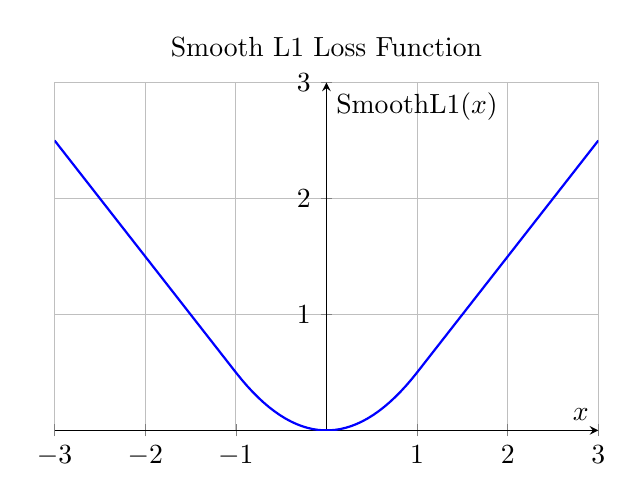
\begin{tikzpicture}
        \begin{axis}[
            title={Smooth L1 Loss Function},
            xlabel={$x$},
            ylabel={SmoothL1($x$)},
            grid=major,
            domain=-3:3, % Bereich der x-Achse
            samples=100, % Anzahl der Punkte
            axis lines=middle, % Achsen durch die Mitte
            %xmin=-3, xmax=3, % Zoom Bereich auf der x-Achse
            width=0.7\textwidth, % Breitere Grafik
            height=6cm, % Schmalere Höhe der Grafik
            ymin=0.0, ymax=3, % Zoom Bereich auf der y-Achse
        ]
            % SmoothL1-Funktion
            \addplot[
                blue, 
                thick
            %]{abs(x) < 0.005 ? 0.5 * (x^2) / 0.005 : abs(x) - 0.5 * 0.005};
            ]{(abs(x) < 1) * (0.5 * x^2) + (abs(x) >= 1) * (abs(x) - 0.5)};
        \end{axis}
    \end{tikzpicture}
    \caption{$SmoothL1$ Loss Funktion}
    \label{fig:smoothL1}
\end{figure}


%%%%%%%%%%%%%%% Setup used for Training CNNs %%%%%%%%%%%%%%%

\section{Setup used for Training CNNs}
\label{sec:trainigsSetup}

% Hardware (GPU, CPU, CUDA)
For training \ac{CNN}s a powerful hardware setup is necessary.
In this work, one main setup is used to train all models.
This work is based on a project proposed and supported by the \ac{ICT} at the \ac{TU}, which also provides the necessary resources.
The department has a server with two NVIDIA Tesla V100S-PCIE-32GB \ac{GPU}s \cite{nvidia_v100_datasheet}.
Since the \ac{GPU}s utilized are equipped with 32 GB of memory and this is sufficient for the needs of this study, all trainings are done on a single \ac{GPU}.
No multi-\ac{GPU} setup is needed.
For this project, CUDA version 12.6 is used, which provides an environment for developing GPU-accelerated applications \cite{nvidia_cuda_126}.
The server employs two Intel(R) Xeon(R) Gold 5118 CPUs @ 2.30GHz \cite{intel_xeon_gold_prozessor_5118}.
These \ac{CPU}s have 24 threads and 12 cores each.

%Weights & Biases

All trainings are logged with the "Weights \& Biases" \cite{wandb}, a developer platform for training and fine-tuning machine learning models.
\cite{wandb} is utilized for logging configurations and results in this work.
The \textit{train loss} and \textit{validation loss} of each training is tracked and visualized in a graph.
The \textit{test \ac{IoU}} and the \textit{best validation loss} are displayed at the end of each training.
Additionally, the \ac{GPU}'s power usage and allocated memory are tracked and graphs are plotted.
Moreover, "Weights \& Biases" \cite{wandb} assigns a unique name to each training session, a critical feature when starting hundreds of training sessions.
All training logs are available at \href{https://wandb.ai/sebiorganization/train-ego-path-detection}{\texttt{https://wandb.ai/sebiorganization/train-ego-path-detection}}.

%PyTorch beschreiben

%%%%%%%% Measuing Inference on NVIDIA Jetson Device %%%%%%%%

\section{Measuing Inference on NVIDIA Jetson Device}
\label{sec:measuringInference}

Due to the nature of this work's use case and potential applications for the system encompassing safety features or preprocessing steps for autonomous trains, the system has to ensure real-time capability when deployed on embedded devices. 
In more detail, one goal for the train track prediction is to be deployed on an Nvidia Jetson device, because of their high computing power and their low power consumption.
Additionally, through NVIDIA's software ecosystem, rapid deployment and latency measurements are possible.
Jetson devices are suitable for applications in autonomous systems and computer vision tasks \cite{nvidia_jetson_embedded_devices}.
Furthermore, the NVIDIA Jetson series is specifically built for machine learning applications, because the devices have \ac{DLA}s built in.
\ac{DLA}s are tensor processor units designed to accelerate the inference of neuronal networks \cite{nvidia_dlas}.

\subsection{Hardware Setup for Measuring Inference}

For this study, the NVIDIA Jetson AGX Xavier is chosen because of several reasons.
This platform achieves up to 32 TOPS by utilizing a \ac{GPU} with 512 cores and 64 Tensor cores, which is advantageous for parallel data processing and neural network inference \cite{nvidia_jetson_agx_xavier_datasheet}.
An additional advantage present the two built-in \ac{NVDLA}s of the AGX Xavier.
\ac{NVDLA}s are NVIDIAs own \ac{DLA}s.
Even though there are more powerful devices like some of the NVIDIA Jetson Orin series, the AGX Xavier is sufficient for this application and cheaper \cite{nvidia_jetson_embedded_devices_prices}.
Additionally, the Xavier has a lower power consumption than the Orin.
Finally but yet important is the ease of integration.
Since, track prediction is a use case of a company, that most commonly uses the Jetson AGX Xavier platform.
Conducting tests on this specific device is appropriate.
The technical specifications of the NVIDIA Jetson AGX Xavier are shown in table \ref{tab:jetson_AGX_xavier_specs}.

\begin{table}[H]
    \centering
    \begin{tabular}{|l|l|}
    %\begin{tabular}{| p{0.3\linewidth} | p{0.6\linewidth} |}
        \hline
        AI Performance & 32 TOPS\\
        \hline
        \ac{GPU} & 512-core NVIDIA Volta GPU with 64 Tensor Cores\\
        \hline
        \ac{CPU} & 8-core NVIDIA Carmel ARM v8.2 64-bit CPU | 8 MB L2 + 4 MB L3\\
        \hline
        Memory & 32 GB 256-Bit LPDDR4x | 136.5 GB/s\\
        \hline
        Storage & 32 GB eMMC 5.1\\
        \hline
        DL Accelerator & (2x) NVDLA\\
        \hline
        Power & 10 W - 30 W\\
        \hline
    \end{tabular}
    \caption{Jetson AGX Xavier technical specifications \cite{nvidia_jetson_agx_xavier_datasheet}}
    \label{tab:jetson_AGX_xavier_specs}
\end{table}

\subsection{Optimizing models with TensorRT}

To fully leverage the used hardware platform Jetson AGX Xavier, NVIDIA introduced TensorRT \cite{nvidia_tensorrt}.
This ecosystem is developed to allow faster inference times when deploying deep learning models.
Also, the baseline paper \cite{tepNet2024} demonstrates through latency measurements that TensorRT consistently outperforms PyTorch in the context of speed.
TensorRT is approximately six times faster than PyTorch, which aligns with the claims made by NVIDIA \cite{tepNet2024} \cite{nvidia_tensorrt}.
Consequently, all latency measurements in this study are conducted using TensorRT.
This framework optimizes inference with methods like quantization, layer and tensor fusion, and kernel tuning \cite{nvidia_tensorrt}.
This can be done for various types of NVIDIA \ac{GPU}s.

\vspace{0.8cm}

\noindent\textbf{Quantization} can optimize an already trained model.
This technique shows a small reduction in accuracy but minimizes latency significantly.
While PyTorch uses PF32 for the inference of its standard models, TensorRT allows to use \ac{GPU}s and \ac{TPU}s to their maximum capacity by permitting FP8, INT8, and INT4.

\vspace{0.8cm}

\noindent\textbf{Layer and Tensor fusion} are used from TensorRT for further optimizing inference.
Often specific layer sequences include two consecutive layers that can be mathematically combined into a single layer.
Resulting in a reduction of unessential computations.

\vspace{0.8cm}

\noindent\textbf{Kernal tuning} is a process that seeks the optimal configuration of available kernels in the Jetson device.
The selected kernels depend on the specific machine-learning application and the used device.
In more detail, the model is executed on the device several times using different CUDA kernels in each run and the best combination is utilized.
Since, Kernel tuning is an iterative process it usually takes a couple of minutes even with compact models.

\subsubsection{TensorRT engine from PyTorch model}

Since TensorRT does not support PyTorch models, a workaround has to be made.
First, the PyTorch models are converted into an \ac{ONNX} format \cite{onnx_docu}.
After that, the \texttt{.onnx} files are optimized by TensorRT with the techniques mentioned before.

\vspace{0.8cm}

\ac{ONNX} is an approach for easier access to hardware optimization and to make interoperability possible \cite{onnx_docu}.
Often machine learning applications are locked in the framework they are developed in, which can present some hurdles.
The \ac{ONNX} format aims for a standardized representation of machine learning models and is therefore commonly used in the community.
Once converted to ONNX, a model utilizes standard data types and a set of built-in operators.
The \ac{ONNX} format version, known as the "opset", defines which operators are used \cite{onnx_docu}.
Therefore the TensorRT version must be compatible with the \ac{ONNX} opset number.

\vspace{0.8cm}

The TensorRT version installed on the Jetson AGX Xavier must support the used \ac{ONNX} opset.
Therefore in this work, the opset 11 is used for all model exports.

\begin{listing}[H]
\begin{minted}[
    frame=single,
    framesep=2mm,
    baselinestretch=1.2,
    bgcolor=white,
    fontsize=\footnotesize,
    linenos
    ]{python}
# Export the model to ONNX
torch.onnx.export(
    model,                       # Model to be exported
    input_tensor,                # Input to the model
    "onnx_file_path/model.onnx", # Output file path
    opset_version=11,            # ONNX version to export the model to
    export_params=True,          # Store the trained parameter
                                 # weights inside the model file
)
\end{minted}
\caption{Exporting a PyTorch model to \ac{ONNX} format}
\label{code:export_model_onnx}
\end{listing}

In this work, all PyTorch models are converted to \texttt{.onnx} files with the built-in torch exporter.
\autoref{code:export_model_onnx} shows that the conversion is done with a single \texttt{torch.onnx.export()} python line \cite{pytorch_onnx_exporter_docu}.
After an \ac{ONNX} model format is created it can be optimized by TensorRT.
This can be executed with the \texttt{trtexec} console application.

\vspace{0.5cm}
\begin{center}
    \texttt{trtexec --onnx=model.onnx --saveEngine=model.engine}
\end{center}
\vspace{0.5cm}

This command provides an example, in which the model.onnx is optimized with TensorRT techniques mentioned above.
Furthermore, the \texttt{model.engine} is saved and can be executed from now on without the need to create it again.
After a couple of minutes, TensorRT outputs a performance summary with many different latencies, like the min, max, mean, or median.
Of these values, the median inference time is considered as the final latency rather than the mean, because it is more robust against outliers.

%%%%%%%%%%%%%%%%%%%%%%%%%%%%%%%%%%%%%%%%%%%%%%%%%%%%%%%%%%%%